\PassOptionsToPackage{unicode=true}{hyperref} % options for packages loaded elsewhere
\PassOptionsToPackage{hyphens}{url}
%
\documentclass[ignorenonframetext,]{beamer}
\usepackage{pgfpages}
\setbeamertemplate{caption}[numbered]
\setbeamertemplate{caption label separator}{: }
\setbeamercolor{caption name}{fg=normal text.fg}
\beamertemplatenavigationsymbolsempty
% Prevent slide breaks in the middle of a paragraph:
\widowpenalties 1 10000
\raggedbottom
\setbeamertemplate{part page}{
\centering
\begin{beamercolorbox}[sep=16pt,center]{part title}
  \usebeamerfont{part title}\insertpart\par
\end{beamercolorbox}
}
\setbeamertemplate{section page}{
\centering
\begin{beamercolorbox}[sep=12pt,center]{part title}
  \usebeamerfont{section title}\insertsection\par
\end{beamercolorbox}
}
\setbeamertemplate{subsection page}{
\centering
\begin{beamercolorbox}[sep=8pt,center]{part title}
  \usebeamerfont{subsection title}\insertsubsection\par
\end{beamercolorbox}
}
\AtBeginPart{
  \frame{\partpage}
}
\AtBeginSection{
  \ifbibliography
  \else
    \frame{\sectionpage}
  \fi
}
\AtBeginSubsection{
  \frame{\subsectionpage}
}
\usepackage{lmodern}
\usepackage{amssymb,amsmath}
\usepackage{ifxetex,ifluatex}
\usepackage{fixltx2e} % provides \textsubscript
\ifnum 0\ifxetex 1\fi\ifluatex 1\fi=0 % if pdftex
  \usepackage[T1]{fontenc}
  \usepackage[utf8]{inputenc}
  \usepackage{textcomp} % provides euro and other symbols
\else % if luatex or xelatex
  \usepackage{unicode-math}
  \defaultfontfeatures{Ligatures=TeX,Scale=MatchLowercase}
\fi
% use upquote if available, for straight quotes in verbatim environments
\IfFileExists{upquote.sty}{\usepackage{upquote}}{}
% use microtype if available
\IfFileExists{microtype.sty}{%
\usepackage[]{microtype}
\UseMicrotypeSet[protrusion]{basicmath} % disable protrusion for tt fonts
}{}
\IfFileExists{parskip.sty}{%
\usepackage{parskip}
}{% else
\setlength{\parindent}{0pt}
\setlength{\parskip}{6pt plus 2pt minus 1pt}
}
\usepackage{hyperref}
\hypersetup{
            pdftitle={Introduction to R Programming},
            pdfauthor={Pedro Fonseca},
            pdfborder={0 0 0},
            breaklinks=true}
\urlstyle{same}  % don't use monospace font for urls
\newif\ifbibliography
\usepackage{color}
\usepackage{fancyvrb}
\newcommand{\VerbBar}{|}
\newcommand{\VERB}{\Verb[commandchars=\\\{\}]}
\DefineVerbatimEnvironment{Highlighting}{Verbatim}{commandchars=\\\{\}}
% Add ',fontsize=\small' for more characters per line
\usepackage{framed}
\definecolor{shadecolor}{RGB}{248,248,248}
\newenvironment{Shaded}{\begin{snugshade}}{\end{snugshade}}
\newcommand{\AlertTok}[1]{\textcolor[rgb]{0.94,0.16,0.16}{#1}}
\newcommand{\AnnotationTok}[1]{\textcolor[rgb]{0.56,0.35,0.01}{\textbf{\textit{#1}}}}
\newcommand{\AttributeTok}[1]{\textcolor[rgb]{0.77,0.63,0.00}{#1}}
\newcommand{\BaseNTok}[1]{\textcolor[rgb]{0.00,0.00,0.81}{#1}}
\newcommand{\BuiltInTok}[1]{#1}
\newcommand{\CharTok}[1]{\textcolor[rgb]{0.31,0.60,0.02}{#1}}
\newcommand{\CommentTok}[1]{\textcolor[rgb]{0.56,0.35,0.01}{\textit{#1}}}
\newcommand{\CommentVarTok}[1]{\textcolor[rgb]{0.56,0.35,0.01}{\textbf{\textit{#1}}}}
\newcommand{\ConstantTok}[1]{\textcolor[rgb]{0.00,0.00,0.00}{#1}}
\newcommand{\ControlFlowTok}[1]{\textcolor[rgb]{0.13,0.29,0.53}{\textbf{#1}}}
\newcommand{\DataTypeTok}[1]{\textcolor[rgb]{0.13,0.29,0.53}{#1}}
\newcommand{\DecValTok}[1]{\textcolor[rgb]{0.00,0.00,0.81}{#1}}
\newcommand{\DocumentationTok}[1]{\textcolor[rgb]{0.56,0.35,0.01}{\textbf{\textit{#1}}}}
\newcommand{\ErrorTok}[1]{\textcolor[rgb]{0.64,0.00,0.00}{\textbf{#1}}}
\newcommand{\ExtensionTok}[1]{#1}
\newcommand{\FloatTok}[1]{\textcolor[rgb]{0.00,0.00,0.81}{#1}}
\newcommand{\FunctionTok}[1]{\textcolor[rgb]{0.00,0.00,0.00}{#1}}
\newcommand{\ImportTok}[1]{#1}
\newcommand{\InformationTok}[1]{\textcolor[rgb]{0.56,0.35,0.01}{\textbf{\textit{#1}}}}
\newcommand{\KeywordTok}[1]{\textcolor[rgb]{0.13,0.29,0.53}{\textbf{#1}}}
\newcommand{\NormalTok}[1]{#1}
\newcommand{\OperatorTok}[1]{\textcolor[rgb]{0.81,0.36,0.00}{\textbf{#1}}}
\newcommand{\OtherTok}[1]{\textcolor[rgb]{0.56,0.35,0.01}{#1}}
\newcommand{\PreprocessorTok}[1]{\textcolor[rgb]{0.56,0.35,0.01}{\textit{#1}}}
\newcommand{\RegionMarkerTok}[1]{#1}
\newcommand{\SpecialCharTok}[1]{\textcolor[rgb]{0.00,0.00,0.00}{#1}}
\newcommand{\SpecialStringTok}[1]{\textcolor[rgb]{0.31,0.60,0.02}{#1}}
\newcommand{\StringTok}[1]{\textcolor[rgb]{0.31,0.60,0.02}{#1}}
\newcommand{\VariableTok}[1]{\textcolor[rgb]{0.00,0.00,0.00}{#1}}
\newcommand{\VerbatimStringTok}[1]{\textcolor[rgb]{0.31,0.60,0.02}{#1}}
\newcommand{\WarningTok}[1]{\textcolor[rgb]{0.56,0.35,0.01}{\textbf{\textit{#1}}}}
\usepackage{graphicx,grffile}
\makeatletter
\def\maxwidth{\ifdim\Gin@nat@width>\linewidth\linewidth\else\Gin@nat@width\fi}
\def\maxheight{\ifdim\Gin@nat@height>\textheight\textheight\else\Gin@nat@height\fi}
\makeatother
% Scale images if necessary, so that they will not overflow the page
% margins by default, and it is still possible to overwrite the defaults
% using explicit options in \includegraphics[width, height, ...]{}
\setkeys{Gin}{width=\maxwidth,height=\maxheight,keepaspectratio}
\setlength{\emergencystretch}{3em}  % prevent overfull lines
\providecommand{\tightlist}{%
  \setlength{\itemsep}{0pt}\setlength{\parskip}{0pt}}
\setcounter{secnumdepth}{0}

% set default figure placement to htbp
\makeatletter
\def\fps@figure{htbp}
\makeatother


\title{Introduction to R Programming}
\providecommand{\subtitle}[1]{}
\subtitle{Data Frames}
\author{Pedro Fonseca}
\date{11 Abril 2020}

\begin{document}
\frame{\titlepage}

\begin{frame}[fragile]{Preliminars}
\protect\hypertarget{preliminars}{}

The \texttt{ifelse()} function performs vectorized if-then-else
statments.

\begin{Shaded}
\begin{Highlighting}[]
\KeywordTok{ifelse}\NormalTok{(test, x, y)}
\end{Highlighting}
\end{Shaded}

\begin{itemize}
\item
  \texttt{test} can be anything that returns a logical vector or matrix
\item
  \texttt{ifelse()}returns \texttt{x} in the positions where the
  corresponding element of \texttt{test} is \texttt{TRUE} and \texttt{y}
  in the positions where the corresponding element of \texttt{test} is
  \texttt{FALSE}
\end{itemize}

\end{frame}

\begin{frame}[fragile]{Preliminars}
\protect\hypertarget{preliminars-1}{}

\begin{Shaded}
\begin{Highlighting}[]
\NormalTok{vec <-}\StringTok{ }\DecValTok{1}\OperatorTok{:}\DecValTok{5}
\end{Highlighting}
\end{Shaded}

\begin{Shaded}
\begin{Highlighting}[]
\KeywordTok{ifelse}\NormalTok{(vec }\OperatorTok{>}\StringTok{ }\DecValTok{2}\NormalTok{, }\DecValTok{2}\NormalTok{, }\DecValTok{1}\NormalTok{)}
\end{Highlighting}
\end{Shaded}

\begin{verbatim}
## [1] 1 1 2 2 2
\end{verbatim}

\begin{Shaded}
\begin{Highlighting}[]
\KeywordTok{ifelse}\NormalTok{(vec }\OperatorTok{>}\StringTok{ }\DecValTok{2}\NormalTok{, }\StringTok{"large"}\NormalTok{, }\StringTok{"small"}\NormalTok{)}
\end{Highlighting}
\end{Shaded}

\begin{verbatim}
## [1] "small" "small" "large" "large" "large"
\end{verbatim}

\begin{Shaded}
\begin{Highlighting}[]
\KeywordTok{ifelse}\NormalTok{(vec }\OperatorTok{>}\StringTok{ }\DecValTok{2}\NormalTok{, vec }\OperatorTok{-}\StringTok{ }\DecValTok{1}\NormalTok{, vec }\OperatorTok{+}\StringTok{ }\DecValTok{1}\NormalTok{)}
\end{Highlighting}
\end{Shaded}

\begin{verbatim}
## [1] 2 3 2 3 4
\end{verbatim}

\end{frame}

\begin{frame}[fragile]{Preliminars}
\protect\hypertarget{preliminars-2}{}

You can chain multiple \texttt{ifelse()} calls:

\begin{Shaded}
\begin{Highlighting}[]
\NormalTok{heights <-}\StringTok{ }\KeywordTok{c}\NormalTok{(}\FloatTok{1.66}\NormalTok{, }\FloatTok{1.88}\NormalTok{, }\FloatTok{1.76}\NormalTok{, }\FloatTok{1.68}\NormalTok{, }\FloatTok{1.7}\NormalTok{, }\FloatTok{1.9}\NormalTok{)}

\NormalTok{shirts <-}\StringTok{ }\KeywordTok{ifelse}\NormalTok{(heights }\OperatorTok{>=}\StringTok{ }\FloatTok{1.9}\NormalTok{, }\StringTok{"XL"}\NormalTok{,}
                 \KeywordTok{ifelse}\NormalTok{(heights }\OperatorTok{>}\StringTok{ }\FloatTok{1.8}\NormalTok{, }\StringTok{"L"}\NormalTok{,}
                        \KeywordTok{ifelse}\NormalTok{(heights }\OperatorTok{>}\StringTok{ }\FloatTok{1.75}\NormalTok{, }\StringTok{"M"}\NormalTok{,}
                               \StringTok{"S"}\NormalTok{)}
\NormalTok{                        )}
\NormalTok{                 )}
\NormalTok{shirts}
\end{Highlighting}
\end{Shaded}

\begin{verbatim}
## [1] "S"  "L"  "M"  "S"  "S"  "XL"
\end{verbatim}

\end{frame}

\begin{frame}{Datasets}
\protect\hypertarget{datasets}{}

In a typical dataset:

\begin{itemize}
\tightlist
\item
  Rows represent observations
\item
  Columns represent variables
\end{itemize}

\begin{figure}
\centering
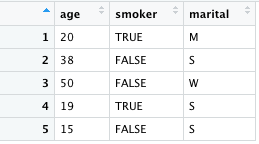
\includegraphics[width=2.08333in,height=\textheight]{dataset}
\caption{A retangular dataset}
\end{figure}

\end{frame}

\begin{frame}{What is a data frame?}
\protect\hypertarget{what-is-a-data-frame}{}

Data frames are designed specifically for retangular datasets.

\begin{itemize}
\item
  Why not matrices? We may need different data types for differen
  columns.
\item
  Why not lists? Not very practical nor visually appealing.
\end{itemize}

\end{frame}

\begin{frame}[fragile]{My first data frame}
\protect\hypertarget{my-first-data-frame}{}

You can create a data frame by supplying name-vector pairs to
\texttt{data.frame()}:

\begin{Shaded}
\begin{Highlighting}[]
\NormalTok{df <-}\StringTok{ }\KeywordTok{data.frame}\NormalTok{(}
\DataTypeTok{age =} \KeywordTok{c}\NormalTok{(}\DecValTok{20}\NormalTok{, }\DecValTok{38}\NormalTok{, }\DecValTok{50}\NormalTok{, }\DecValTok{19}\NormalTok{),}
\DataTypeTok{smoker =} \KeywordTok{c}\NormalTok{(}\OtherTok{TRUE}\NormalTok{, }\OtherTok{FALSE}\NormalTok{, }\OtherTok{FALSE}\NormalTok{, }\OtherTok{FALSE}\NormalTok{),}
\DataTypeTok{marital =} \KeywordTok{factor}\NormalTok{(}\KeywordTok{c}\NormalTok{(}\StringTok{"M"}\NormalTok{, }\StringTok{"S"}\NormalTok{, }\StringTok{"W"}\NormalTok{, }\StringTok{"S"}\NormalTok{))}
\NormalTok{)}
\NormalTok{df}
\end{Highlighting}
\end{Shaded}

\begin{verbatim}
##   age smoker marital
## 1  20   TRUE       M
## 2  38  FALSE       S
## 3  50  FALSE       W
## 4  19  FALSE       S
\end{verbatim}

Data frame rows are numbered by default.

\end{frame}

\begin{frame}[fragile]{Some utilities}
\protect\hypertarget{some-utilities}{}

\begin{Shaded}
\begin{Highlighting}[]
\KeywordTok{summary}\NormalTok{(df)}
\end{Highlighting}
\end{Shaded}

\begin{verbatim}
##       age          smoker        marital
##  Min.   :19.00   Mode :logical   M:1    
##  1st Qu.:19.75   FALSE:3         S:2    
##  Median :29.00   TRUE :1         W:1    
##  Mean   :31.75                          
##  3rd Qu.:41.00                          
##  Max.   :50.00
\end{verbatim}

Try this:

\begin{Shaded}
\begin{Highlighting}[]
\KeywordTok{View}\NormalTok{(df)}
\end{Highlighting}
\end{Shaded}

\end{frame}

\begin{frame}[fragile]{What is a data frame?}
\protect\hypertarget{what-is-a-data-frame-1}{}

\begin{Shaded}
\begin{Highlighting}[]
\KeywordTok{str}\NormalTok{(df)}
\end{Highlighting}
\end{Shaded}

\begin{verbatim}
## 'data.frame':    4 obs. of  3 variables:
##  $ age    : num  20 38 50 19
##  $ smoker : logi  TRUE FALSE FALSE FALSE
##  $ marital: Factor w/ 3 levels "M","S","W": 1 2 3 2
\end{verbatim}

\begin{itemize}
\tightlist
\item
  Similar to the structure of a list?
\item
  Actually, data frames are build on top of lists.
\item
  A data frame is a list of atomic vectors with equal length.
\end{itemize}

\end{frame}

\begin{frame}[fragile]{What is a data frame?}
\protect\hypertarget{what-is-a-data-frame-2}{}

A data frame is a named list of vectors with attributes for column
\texttt{names}, \texttt{row.names}, and its own class:

\begin{Shaded}
\begin{Highlighting}[]
\KeywordTok{typeof}\NormalTok{(df) }
\end{Highlighting}
\end{Shaded}

\begin{verbatim}
## [1] "list"
\end{verbatim}

\begin{Shaded}
\begin{Highlighting}[]
\KeywordTok{class}\NormalTok{(df) }
\end{Highlighting}
\end{Shaded}

\begin{verbatim}
## [1] "data.frame"
\end{verbatim}

\end{frame}

\begin{frame}[fragile]{What is a data frame?}
\protect\hypertarget{what-is-a-data-frame-3}{}

Due to their rectangular scructure, data frames share the properties of
both matrices and lists:

\begin{itemize}
\item
  A data frame has \texttt{rownames()} and \texttt{colnames()}. The
  \texttt{names()} of a data frame are the column names.
\item
  A data frame has \texttt{nrow()} rows and \texttt{ncol()} columns.
  \texttt{The\ length()} of a data frame is the number of columns.
\end{itemize}

\end{frame}

\begin{frame}[fragile]{My second data frame}
\protect\hypertarget{my-second-data-frame}{}

\begin{Shaded}
\begin{Highlighting}[]
\NormalTok{name <-}\StringTok{ }\KeywordTok{c}\NormalTok{(}\StringTok{"Anne"}\NormalTok{, }\StringTok{"Pete"}\NormalTok{, }\StringTok{"Frank"}\NormalTok{, }\StringTok{"Julia"}\NormalTok{, }\StringTok{"Cath"}\NormalTok{)}
\NormalTok{age <-}\StringTok{ }\KeywordTok{c}\NormalTok{(}\DecValTok{28}\NormalTok{, }\DecValTok{30}\NormalTok{, }\DecValTok{21}\NormalTok{, }\DecValTok{39}\NormalTok{, }\DecValTok{35}\NormalTok{)}
\NormalTok{child <-}\StringTok{ }\KeywordTok{c}\NormalTok{(}\OtherTok{FALSE}\NormalTok{, }\OtherTok{TRUE}\NormalTok{, }\OtherTok{TRUE}\NormalTok{, }\OtherTok{FALSE}\NormalTok{, }\OtherTok{TRUE}\NormalTok{)}

\NormalTok{df2 <-}\StringTok{ }\KeywordTok{data.frame}\NormalTok{(name, age, child)}
\NormalTok{df2}
\end{Highlighting}
\end{Shaded}

\begin{verbatim}
##    name age child
## 1  Anne  28 FALSE
## 2  Pete  30  TRUE
## 3 Frank  21  TRUE
## 4 Julia  39 FALSE
## 5  Cath  35  TRUE
\end{verbatim}

Unlike \texttt{list()}, \texttt{data.frame()} keeps the names of the
vectors.

\end{frame}

\begin{frame}[fragile]{Assign \texttt{names()} to a data frame}
\protect\hypertarget{assign-names-to-a-data-frame}{}

Data frame columns always have names. If you dont provide them, default
names will be assigned:

\begin{Shaded}
\begin{Highlighting}[]
\NormalTok{df3 <-}\StringTok{ }\KeywordTok{data.frame}\NormalTok{(}
  \KeywordTok{c}\NormalTok{(}\DecValTok{1}\NormalTok{, }\DecValTok{4}\NormalTok{, }\DecValTok{6}\NormalTok{),}
  \KeywordTok{c}\NormalTok{(}\DecValTok{6}\NormalTok{, }\DecValTok{7}\NormalTok{, }\DecValTok{9}\NormalTok{)}
\NormalTok{) }

\NormalTok{df3}
\end{Highlighting}
\end{Shaded}

\begin{verbatim}
##   c.1..4..6. c.6..7..9.
## 1          1          6
## 2          4          7
## 3          6          9
\end{verbatim}

\end{frame}

\begin{frame}[fragile]{Assign \texttt{names()} to a data frame}
\protect\hypertarget{assign-names-to-a-data-frame-1}{}

\begin{Shaded}
\begin{Highlighting}[]
\KeywordTok{names}\NormalTok{(df3) <-}\StringTok{ }\KeywordTok{c}\NormalTok{(}\StringTok{"a-name"}\NormalTok{, }\StringTok{"some-other-name"}\NormalTok{)}
\NormalTok{df3}
\end{Highlighting}
\end{Shaded}

\begin{verbatim}
##   a-name some-other-name
## 1      1               6
## 2      4               7
## 3      6               9
\end{verbatim}

\end{frame}

\begin{frame}[fragile]{Row names}
\protect\hypertarget{row-names}{}

\texttt{data.frame()} allows you to label row indexes. You can provide a
vector of unique values to the \texttt{row.names} argument:

\begin{Shaded}
\begin{Highlighting}[]
\NormalTok{df4 <-}\StringTok{ }\KeywordTok{data.frame}\NormalTok{(}
  \DataTypeTok{age =} \KeywordTok{c}\NormalTok{(}\DecValTok{35}\NormalTok{, }\DecValTok{27}\NormalTok{, }\DecValTok{18}\NormalTok{),}
  \DataTypeTok{hair =} \KeywordTok{c}\NormalTok{(}\StringTok{"blond"}\NormalTok{, }\StringTok{"brown"}\NormalTok{, }\StringTok{"black"}\NormalTok{),}
  \DataTypeTok{row.names =} \KeywordTok{c}\NormalTok{(}\StringTok{"Bob"}\NormalTok{, }\StringTok{"Susan"}\NormalTok{, }\StringTok{"Sam"}\NormalTok{) }\CommentTok{# row names!}
\NormalTok{) }

\NormalTok{df4}
\end{Highlighting}
\end{Shaded}

\begin{verbatim}
##       age  hair
## Bob    35 blond
## Susan  27 brown
## Sam    18 black
\end{verbatim}

\begin{Shaded}
\begin{Highlighting}[]
\KeywordTok{rownames}\NormalTok{(df4)}
\end{Highlighting}
\end{Shaded}

\begin{verbatim}
## [1] "Bob"   "Susan" "Sam"
\end{verbatim}

\end{frame}

\begin{frame}[fragile]{Row names}
\protect\hypertarget{row-names-1}{}

You can also set (or ovewright) row names after the data frame is
created:

\begin{Shaded}
\begin{Highlighting}[]
\KeywordTok{rownames}\NormalTok{(df4) <-}\StringTok{ }\KeywordTok{c}\NormalTok{(}\StringTok{"Bob M."}\NormalTok{, }\StringTok{"Susab B."}\NormalTok{, }\StringTok{"Sam L."}\NormalTok{) }
\NormalTok{df4}
\end{Highlighting}
\end{Shaded}

\begin{verbatim}
##          age  hair
## Bob M.    35 blond
## Susab B.  27 brown
## Sam L.    18 black
\end{verbatim}

\end{frame}

\begin{frame}[fragile]{\texttt{stringsAsFactors}}
\protect\hypertarget{stringsasfactors}{}

\begin{Shaded}
\begin{Highlighting}[]
\NormalTok{df5 <-}\StringTok{ }\KeywordTok{data.frame}\NormalTok{(}
  \DataTypeTok{person =} \KeywordTok{c}\NormalTok{(}\StringTok{"John"}\NormalTok{, }\StringTok{"Matt"}\NormalTok{, }\StringTok{"Mary"}\NormalTok{),}
  \DataTypeTok{age =} \KeywordTok{c}\NormalTok{(}\DecValTok{20}\NormalTok{, }\DecValTok{38}\NormalTok{, }\DecValTok{50}\NormalTok{),}
  \DataTypeTok{smoker =} \KeywordTok{c}\NormalTok{(}\OtherTok{TRUE}\NormalTok{, }\OtherTok{FALSE}\NormalTok{, }\OtherTok{FALSE}\NormalTok{),}
  \DataTypeTok{marital =} \KeywordTok{factor}\NormalTok{(}\KeywordTok{c}\NormalTok{(}\StringTok{"M"}\NormalTok{, }\StringTok{"S"}\NormalTok{, }\StringTok{"S"}\NormalTok{))}
\NormalTok{)}

\KeywordTok{str}\NormalTok{(df5)}
\end{Highlighting}
\end{Shaded}

\begin{verbatim}
## 'data.frame':    3 obs. of  4 variables:
##  $ person : Factor w/ 3 levels "John","Mary",..: 1 3 2
##  $ age    : num  20 38 50
##  $ smoker : logi  TRUE FALSE FALSE
##  $ marital: Factor w/ 2 levels "M","S": 1 2 2
\end{verbatim}

The \texttt{person} variable is a factor! Why?

\end{frame}

\begin{frame}[fragile]{stringsAsFactors}
\protect\hypertarget{stringsasfactors-1}{}

The \texttt{stringsAsFactors} argument of \texttt{data.frame} is set to
\texttt{TRUE} by default.

\begin{Shaded}
\begin{Highlighting}[]
\NormalTok{df6 <-}\StringTok{ }\KeywordTok{data.frame}\NormalTok{(}
  \DataTypeTok{person =} \KeywordTok{c}\NormalTok{(}\StringTok{"John"}\NormalTok{, }\StringTok{"Matt"}\NormalTok{, }\StringTok{"Mary"}\NormalTok{),}
  \DataTypeTok{age =} \KeywordTok{c}\NormalTok{(}\DecValTok{20}\NormalTok{, }\DecValTok{38}\NormalTok{, }\DecValTok{50}\NormalTok{),}
  \DataTypeTok{smoker =} \KeywordTok{c}\NormalTok{(}\OtherTok{TRUE}\NormalTok{, }\OtherTok{FALSE}\NormalTok{, }\OtherTok{FALSE}\NormalTok{),}
  \DataTypeTok{marital =} \KeywordTok{factor}\NormalTok{(}\KeywordTok{c}\NormalTok{(}\StringTok{"M"}\NormalTok{, }\StringTok{"S"}\NormalTok{, }\StringTok{"S"}\NormalTok{)),}
  \DataTypeTok{stringsAsFactors =} \OtherTok{FALSE}
\NormalTok{)}
\KeywordTok{str}\NormalTok{(df6)}
\end{Highlighting}
\end{Shaded}

\begin{verbatim}
## 'data.frame':    3 obs. of  4 variables:
##  $ person : chr  "John" "Matt" "Mary"
##  $ age    : num  20 38 50
##  $ smoker : logi  TRUE FALSE FALSE
##  $ marital: Factor w/ 2 levels "M","S": 1 2 2
\end{verbatim}

\end{frame}

\begin{frame}[fragile]{Testing and coercing}
\protect\hypertarget{testing-and-coercing}{}

To check if an object is a data frame use \texttt{is.data.frame()}:

\begin{Shaded}
\begin{Highlighting}[]
\KeywordTok{is.data.frame}\NormalTok{(df6)}
\end{Highlighting}
\end{Shaded}

\begin{verbatim}
## [1] TRUE
\end{verbatim}

You can coerce an object to a data frame with \texttt{as.data.frame()}:

\begin{Shaded}
\begin{Highlighting}[]
\NormalTok{M <-}\StringTok{ }\KeywordTok{matrix}\NormalTok{(}\DecValTok{1}\OperatorTok{:}\DecValTok{9}\NormalTok{, }\DataTypeTok{ncol =} \DecValTok{3}\NormalTok{)}
\KeywordTok{as.data.frame}\NormalTok{(M)}
\end{Highlighting}
\end{Shaded}

\begin{verbatim}
##   V1 V2 V3
## 1  1  4  7
## 2  2  5  8
## 3  3  6  9
\end{verbatim}

\end{frame}

\begin{frame}{Subsetting}
\protect\hypertarget{subsetting}{}

Data frames inherit subsetting syntax from both matrices and lists. You
can subset a data frame:

\begin{itemize}
\tightlist
\item
  Like a 2D structure (behaves like a matrix)
\item
  Like a 1D structure (behaves like a list)
\end{itemize}

\end{frame}

\begin{frame}[fragile]{Subsetting}
\protect\hypertarget{subsetting-1}{}

\begin{Shaded}
\begin{Highlighting}[]
\NormalTok{name <-}\StringTok{ }\KeywordTok{c}\NormalTok{(}\StringTok{"Anne"}\NormalTok{, }\StringTok{"Pete"}\NormalTok{, }\StringTok{"Frank"}\NormalTok{, }\StringTok{"Julia"}\NormalTok{, }\StringTok{"Cath"}\NormalTok{) }
\NormalTok{age <-}\StringTok{ }\KeywordTok{c}\NormalTok{(}\DecValTok{28}\NormalTok{, }\DecValTok{30}\NormalTok{, }\DecValTok{21}\NormalTok{, }\DecValTok{39}\NormalTok{, }\OtherTok{NA}\NormalTok{)}
\NormalTok{child <-}\StringTok{ }\KeywordTok{c}\NormalTok{(}\OtherTok{FALSE}\NormalTok{, }\OtherTok{FALSE}\NormalTok{, }\OtherTok{TRUE}\NormalTok{, }\OtherTok{FALSE}\NormalTok{, }\OtherTok{TRUE}\NormalTok{)}

\NormalTok{people <-}\StringTok{ }\KeywordTok{data.frame}\NormalTok{(name, age, child, }
                     \DataTypeTok{stringsAsFactors =} \OtherTok{FALSE}\NormalTok{)}
\NormalTok{people}
\end{Highlighting}
\end{Shaded}

\begin{verbatim}
##    name age child
## 1  Anne  28 FALSE
## 2  Pete  30 FALSE
## 3 Frank  21  TRUE
## 4 Julia  39 FALSE
## 5  Cath  NA  TRUE
\end{verbatim}

\end{frame}

\begin{frame}[fragile]{Subsetting with matrix syntax}
\protect\hypertarget{subsetting-with-matrix-syntax}{}

\begin{Shaded}
\begin{Highlighting}[]
\NormalTok{people[}\DecValTok{3}\NormalTok{, ] }\CommentTok{# returns a data frame}
\end{Highlighting}
\end{Shaded}

\begin{verbatim}
##    name age child
## 3 Frank  21  TRUE
\end{verbatim}

\begin{Shaded}
\begin{Highlighting}[]
\NormalTok{people[}\KeywordTok{c}\NormalTok{(}\DecValTok{1}\NormalTok{, }\DecValTok{3}\NormalTok{), ] }\CommentTok{# data frame}
\end{Highlighting}
\end{Shaded}

\begin{verbatim}
##    name age child
## 1  Anne  28 FALSE
## 3 Frank  21  TRUE
\end{verbatim}

\begin{Shaded}
\begin{Highlighting}[]
\NormalTok{people[}\DecValTok{3}\NormalTok{, }\DecValTok{2}\NormalTok{] }\CommentTok{# vector}
\end{Highlighting}
\end{Shaded}

\begin{verbatim}
## [1] 21
\end{verbatim}

\begin{Shaded}
\begin{Highlighting}[]
\NormalTok{people[}\DecValTok{3}\NormalTok{, }\StringTok{"age"}\NormalTok{] }\CommentTok{# vector}
\end{Highlighting}
\end{Shaded}

\begin{verbatim}
## [1] 21
\end{verbatim}

\end{frame}

\begin{frame}[fragile]{Subsetting with matrix syntax}
\protect\hypertarget{subsetting-with-matrix-syntax-1}{}

\begin{Shaded}
\begin{Highlighting}[]
\NormalTok{people[, }\StringTok{"age"}\NormalTok{] }\CommentTok{# vector}
\end{Highlighting}
\end{Shaded}

\begin{verbatim}
## [1] 28 30 21 39 NA
\end{verbatim}

\begin{Shaded}
\begin{Highlighting}[]
\NormalTok{people[, }\DecValTok{1}\NormalTok{] }\CommentTok{#  vector}
\end{Highlighting}
\end{Shaded}

\begin{verbatim}
## [1] "Anne"  "Pete"  "Frank" "Julia" "Cath"
\end{verbatim}

\begin{Shaded}
\begin{Highlighting}[]
\NormalTok{people[}\KeywordTok{c}\NormalTok{(}\DecValTok{3}\NormalTok{, }\DecValTok{5}\NormalTok{), }\KeywordTok{c}\NormalTok{(}\StringTok{"age"}\NormalTok{, }\StringTok{"child"}\NormalTok{)] }\CommentTok{# data frame}
\end{Highlighting}
\end{Shaded}

\begin{verbatim}
##   age child
## 3  21  TRUE
## 5  NA  TRUE
\end{verbatim}

\end{frame}

\begin{frame}[fragile]{Subsetting with matrix syntax}
\protect\hypertarget{subsetting-with-matrix-syntax-2}{}

See the pattern?

\begin{itemize}
\item
  When you subset a dataframe like a 2D object with \texttt{{[}} you get
  a vector if only one column is extracted. You get a data frame
  otherwise.
\item
  This is a frequent source of bugs when using \texttt{{[}} in a
  function, unless you always remember to use \texttt{drop\ =\ FALSE}.
\end{itemize}

\end{frame}

\begin{frame}[fragile]{Subsetting with matrix syntax}
\protect\hypertarget{subsetting-with-matrix-syntax-3}{}

\begin{Shaded}
\begin{Highlighting}[]
\NormalTok{people[, }\StringTok{"age"}\NormalTok{, drop =}\StringTok{ }\OtherTok{FALSE}\NormalTok{] }\CommentTok{# data frame!}
\end{Highlighting}
\end{Shaded}

\begin{verbatim}
##   age
## 1  28
## 2  30
## 3  21
## 4  39
## 5  NA
\end{verbatim}

Setting \texttt{drop\ =\ FALSE} prevents \texttt{{[}} from coercing to a
lower dimension.

\end{frame}

\begin{frame}[fragile]{Subsetting with matrix syntax}
\protect\hypertarget{subsetting-with-matrix-syntax-4}{}

You can also subset using logical conditions.

Show \texttt{name} and \texttt{child} for the people with known
\texttt{age}:

\begin{Shaded}
\begin{Highlighting}[]
\NormalTok{people[}\OperatorTok{!}\KeywordTok{is.na}\NormalTok{(people[, }\StringTok{"age"}\NormalTok{]), }\KeywordTok{c}\NormalTok{(}\StringTok{"name"}\NormalTok{, }\StringTok{"child"}\NormalTok{)]}
\end{Highlighting}
\end{Shaded}

\begin{verbatim}
##    name child
## 1  Anne FALSE
## 2  Pete FALSE
## 3 Frank  TRUE
## 4 Julia FALSE
\end{verbatim}

\end{frame}

\begin{frame}[fragile]{Subsetting with matrix syntax}
\protect\hypertarget{subsetting-with-matrix-syntax-5}{}

Show \texttt{name} and \texttt{child} for the people who are older than
21:

\begin{Shaded}
\begin{Highlighting}[]
\NormalTok{people[}\OperatorTok{!}\KeywordTok{is.na}\NormalTok{(people[, }\StringTok{"age"}\NormalTok{]) }\OperatorTok{&}\StringTok{ }\NormalTok{people[, }\StringTok{"age"}\NormalTok{] }\OperatorTok{>}\StringTok{ }\DecValTok{21}\NormalTok{,}
       \KeywordTok{c}\NormalTok{(}\StringTok{"name"}\NormalTok{, }\StringTok{"child"}\NormalTok{)]}
\end{Highlighting}
\end{Shaded}

\begin{verbatim}
##    name child
## 1  Anne FALSE
## 2  Pete FALSE
## 4 Julia FALSE
\end{verbatim}

\end{frame}

\begin{frame}[fragile]{Subsetting with matrix syntax}
\protect\hypertarget{subsetting-with-matrix-syntax-6}{}

If available, row names can be used for subseting:

\begin{Shaded}
\begin{Highlighting}[]
\NormalTok{df4}
\end{Highlighting}
\end{Shaded}

\begin{verbatim}
##          age  hair
## Bob M.    35 blond
## Susab B.  27 brown
## Sam L.    18 black
\end{verbatim}

\begin{Shaded}
\begin{Highlighting}[]
\NormalTok{df4[}\StringTok{"Bob M."}\NormalTok{, ]}
\end{Highlighting}
\end{Shaded}

\begin{verbatim}
##        age  hair
## Bob M.  35 blond
\end{verbatim}

\begin{Shaded}
\begin{Highlighting}[]
\NormalTok{df4[}\StringTok{"Bob M."}\NormalTok{, }\StringTok{"hair"}\NormalTok{]}
\end{Highlighting}
\end{Shaded}

\begin{verbatim}
## [1] blond
## Levels: black blond brown
\end{verbatim}

\end{frame}

\begin{frame}[fragile]{Subsetting with list syntax}
\protect\hypertarget{subsetting-with-list-syntax}{}

\begin{Shaded}
\begin{Highlighting}[]
\NormalTok{people[}\DecValTok{2}\NormalTok{] }\CommentTok{# data frame}
\end{Highlighting}
\end{Shaded}

\begin{verbatim}
##   age
## 1  28
## 2  30
## 3  21
## 4  39
## 5  NA
\end{verbatim}

\begin{Shaded}
\begin{Highlighting}[]
\NormalTok{people[}\StringTok{"age"}\NormalTok{] }\CommentTok{# data frame}
\end{Highlighting}
\end{Shaded}

\begin{verbatim}
##   age
## 1  28
## 2  30
## 3  21
## 4  39
## 5  NA
\end{verbatim}

\end{frame}

\begin{frame}[fragile]{Subsetting with list syntax}
\protect\hypertarget{subsetting-with-list-syntax-1}{}

\begin{Shaded}
\begin{Highlighting}[]
\NormalTok{people[}\KeywordTok{c}\NormalTok{(}\DecValTok{1}\NormalTok{, }\DecValTok{3}\NormalTok{)] }\CommentTok{# data frame}
\end{Highlighting}
\end{Shaded}

\begin{verbatim}
##    name child
## 1  Anne FALSE
## 2  Pete FALSE
## 3 Frank  TRUE
## 4 Julia FALSE
## 5  Cath  TRUE
\end{verbatim}

\begin{Shaded}
\begin{Highlighting}[]
\NormalTok{people[}\KeywordTok{c}\NormalTok{(}\StringTok{"name"}\NormalTok{, }\StringTok{"child"}\NormalTok{)] }\CommentTok{# data frame}
\end{Highlighting}
\end{Shaded}

\begin{verbatim}
##    name child
## 1  Anne FALSE
## 2  Pete FALSE
## 3 Frank  TRUE
## 4 Julia FALSE
## 5  Cath  TRUE
\end{verbatim}

\end{frame}

\begin{frame}[fragile]{Subsetting with list syntax}
\protect\hypertarget{subsetting-with-list-syntax-2}{}

\begin{Shaded}
\begin{Highlighting}[]
\NormalTok{people[}\StringTok{"age"}\NormalTok{] }\CommentTok{# data frame}
\end{Highlighting}
\end{Shaded}

\begin{verbatim}
##   age
## 1  28
## 2  30
## 3  21
## 4  39
## 5  NA
\end{verbatim}

\begin{Shaded}
\begin{Highlighting}[]
\NormalTok{people[[}\StringTok{"age"}\NormalTok{]] }\CommentTok{# vector}
\end{Highlighting}
\end{Shaded}

\begin{verbatim}
## [1] 28 30 21 39 NA
\end{verbatim}

\begin{Shaded}
\begin{Highlighting}[]
\NormalTok{people}\OperatorTok{$}\NormalTok{age }\CommentTok{# vector}
\end{Highlighting}
\end{Shaded}

\begin{verbatim}
## [1] 28 30 21 39 NA
\end{verbatim}

\end{frame}

\begin{frame}[fragile]{Subsetting with list syntax}
\protect\hypertarget{subsetting-with-list-syntax-3}{}

\begin{Shaded}
\begin{Highlighting}[]
\NormalTok{people[[}\StringTok{"age"}\NormalTok{]][}\DecValTok{1}\NormalTok{]}
\end{Highlighting}
\end{Shaded}

\begin{verbatim}
## [1] 28
\end{verbatim}

\begin{Shaded}
\begin{Highlighting}[]
\NormalTok{people[[}\StringTok{"age"}\NormalTok{]][}\KeywordTok{c}\NormalTok{(}\DecValTok{1}\NormalTok{, }\DecValTok{4}\NormalTok{)]}
\end{Highlighting}
\end{Shaded}

\begin{verbatim}
## [1] 28 39
\end{verbatim}

\begin{Shaded}
\begin{Highlighting}[]
\NormalTok{people}\OperatorTok{$}\NormalTok{age[}\DecValTok{1}\NormalTok{]}
\end{Highlighting}
\end{Shaded}

\begin{verbatim}
## [1] 28
\end{verbatim}

\begin{Shaded}
\begin{Highlighting}[]
\NormalTok{people}\OperatorTok{$}\NormalTok{age[}\KeywordTok{c}\NormalTok{(}\DecValTok{1}\NormalTok{, }\DecValTok{4}\NormalTok{)]}
\end{Highlighting}
\end{Shaded}

\begin{verbatim}
## [1] 28 39
\end{verbatim}

\end{frame}

\begin{frame}[fragile]{Subsetting with list syntax}
\protect\hypertarget{subsetting-with-list-syntax-4}{}

\begin{Shaded}
\begin{Highlighting}[]
\NormalTok{people[[}\DecValTok{2}\NormalTok{]] }\CommentTok{# same as people[["age"]]}
\end{Highlighting}
\end{Shaded}

\begin{verbatim}
## [1] 28 30 21 39 NA
\end{verbatim}

\begin{Shaded}
\begin{Highlighting}[]
\NormalTok{people[[}\DecValTok{2}\NormalTok{]][}\DecValTok{1}\NormalTok{]}
\end{Highlighting}
\end{Shaded}

\begin{verbatim}
## [1] 28
\end{verbatim}

\begin{Shaded}
\begin{Highlighting}[]
\NormalTok{people[[}\DecValTok{2}\NormalTok{]][}\KeywordTok{c}\NormalTok{(}\DecValTok{1}\NormalTok{, }\DecValTok{4}\NormalTok{)]}
\end{Highlighting}
\end{Shaded}

\begin{verbatim}
## [1] 28 39
\end{verbatim}

\end{frame}

\begin{frame}[fragile]{Subsetting with list syntax}
\protect\hypertarget{subsetting-with-list-syntax-5}{}

Since data frames are lists of vectors, when you subset a dataframe like
a 1D object:

\begin{itemize}
\tightlist
\item
  with \texttt{{[}} you get a dataframe.
\item
  with \texttt{{[}{[}} or \texttt{\$} you get a vector.
\end{itemize}

\end{frame}

\begin{frame}[fragile]{Partial matching with \texttt{\$}}
\protect\hypertarget{partial-matching-with}{}

When you attempt to extract a column from \texttt{df} with
\texttt{df\$name} and there is no column \texttt{name}, a data frame
will instead select any variable that starts with \texttt{name}. If no
variable starts with \texttt{name} (or if more than one do),
\texttt{df\$name} will return \texttt{NULL}.

\begin{Shaded}
\begin{Highlighting}[]
\KeywordTok{names}\NormalTok{(df)}
\end{Highlighting}
\end{Shaded}

\begin{verbatim}
## [1] "age"     "smoker"  "marital"
\end{verbatim}

\begin{Shaded}
\begin{Highlighting}[]
\NormalTok{df}\OperatorTok{$}\NormalTok{a}
\end{Highlighting}
\end{Shaded}

\begin{verbatim}
## [1] 20 38 50 19
\end{verbatim}

By default, \texttt{{[}{[}} does not do partial matching. Why? Run
\texttt{?"{[}{[}"} and check what is the default value of the
\texttt{exact} argument.

\texttt{df\$name} is equivalent to
\texttt{df{[}{[}"name",\ exact\ =\ FALSE{]}{]}}

\end{frame}

\begin{frame}[fragile]{Add columns with \texttt{\$}}
\protect\hypertarget{add-columns-with}{}

So far our data frame \texttt{people} has 5 rows and 3 columns.

\begin{Shaded}
\begin{Highlighting}[]
\KeywordTok{str}\NormalTok{(people)}
\end{Highlighting}
\end{Shaded}

\begin{verbatim}
## 'data.frame':    5 obs. of  3 variables:
##  $ name : chr  "Anne" "Pete" "Frank" "Julia" ...
##  $ age  : num  28 30 21 39 NA
##  $ child: logi  FALSE FALSE TRUE FALSE TRUE
\end{verbatim}

\end{frame}

\begin{frame}[fragile]{Add columns with \texttt{\$}}
\protect\hypertarget{add-columns-with-1}{}

Let's add a column with the people's heigth:

\begin{Shaded}
\begin{Highlighting}[]
\NormalTok{height <-}\StringTok{ }\KeywordTok{c}\NormalTok{(}\DecValTok{175}\NormalTok{, }\DecValTok{170}\NormalTok{, }\DecValTok{166}\NormalTok{, }\DecValTok{182}\NormalTok{, }\DecValTok{172}\NormalTok{) }
\NormalTok{people}\OperatorTok{$}\NormalTok{height <-}\StringTok{ }\NormalTok{height}

\KeywordTok{str}\NormalTok{(people)}
\end{Highlighting}
\end{Shaded}

\begin{verbatim}
## 'data.frame':    5 obs. of  4 variables:
##  $ name  : chr  "Anne" "Pete" "Frank" "Julia" ...
##  $ age   : num  28 30 21 39 NA
##  $ child : logi  FALSE FALSE TRUE FALSE TRUE
##  $ height: num  175 170 166 182 172
\end{verbatim}

\end{frame}

\begin{frame}[fragile]{Add columns with \texttt{cbind()}}
\protect\hypertarget{add-columns-with-cbind}{}

Now let's add a column with the people's weight:

\begin{Shaded}
\begin{Highlighting}[]
\NormalTok{ weight <-}\StringTok{ }\KeywordTok{c}\NormalTok{(}\DecValTok{86}\NormalTok{, }\DecValTok{63}\NormalTok{, }\DecValTok{68}\NormalTok{, }\DecValTok{55}\NormalTok{, }\DecValTok{56}\NormalTok{)}
\NormalTok{ people <-}\StringTok{ }\KeywordTok{cbind}\NormalTok{(people, weight)}
 
 \KeywordTok{str}\NormalTok{(people)}
\end{Highlighting}
\end{Shaded}

\begin{verbatim}
## 'data.frame':    5 obs. of  5 variables:
##  $ name  : chr  "Anne" "Pete" "Frank" "Julia" ...
##  $ age   : num  28 30 21 39 NA
##  $ child : logi  FALSE FALSE TRUE FALSE TRUE
##  $ height: num  175 170 166 182 172
##  $ weight: num  86 63 68 55 56
\end{verbatim}

\end{frame}

\begin{frame}[fragile]{Modify columns}
\protect\hypertarget{modify-columns}{}

We can overwrite existing columns.

Lets convert \texttt{height} from centimenters to meters:

\begin{Shaded}
\begin{Highlighting}[]
\NormalTok{people}\OperatorTok{$}\NormalTok{height <-}\StringTok{ }\NormalTok{people}\OperatorTok{$}\NormalTok{height}\OperatorTok{/}\DecValTok{100}

\NormalTok{people}
\end{Highlighting}
\end{Shaded}

\begin{verbatim}
##    name age child height weight
## 1  Anne  28 FALSE   1.75     86
## 2  Pete  30 FALSE   1.70     63
## 3 Frank  21  TRUE   1.66     68
## 4 Julia  39 FALSE   1.82     55
## 5  Cath  NA  TRUE   1.72     56
\end{verbatim}

\end{frame}

\begin{frame}[fragile]{Calculations with existing columns}
\protect\hypertarget{calculations-with-existing-columns}{}

We can create new colums using the values of existing columns.

Let's use \texttt{weight} and \texttt{height} to calculate the body mass
index:

\begin{Shaded}
\begin{Highlighting}[]
\NormalTok{people}\OperatorTok{$}\NormalTok{bmi <-}\StringTok{ }\KeywordTok{round}\NormalTok{(}
\NormalTok{  people}\OperatorTok{$}\NormalTok{weight}\OperatorTok{/}\NormalTok{((people}\OperatorTok{$}\NormalTok{height)}\OperatorTok{^}\DecValTok{2}\NormalTok{)}
\NormalTok{  )}
\NormalTok{people}
\end{Highlighting}
\end{Shaded}

\begin{verbatim}
##    name age child height weight bmi
## 1  Anne  28 FALSE   1.75     86  28
## 2  Pete  30 FALSE   1.70     63  22
## 3 Frank  21  TRUE   1.66     68  25
## 4 Julia  39 FALSE   1.82     55  17
## 5  Cath  NA  TRUE   1.72     56  19
\end{verbatim}

\end{frame}

\begin{frame}[fragile]{Calculations with existing columns}
\protect\hypertarget{calculations-with-existing-columns-1}{}

Now let's the the body mass index to calculate the weigth status:

\begin{Shaded}
\begin{Highlighting}[]
\NormalTok{people}\OperatorTok{$}\NormalTok{weight_status <-}\StringTok{ }\KeywordTok{ifelse}\NormalTok{(}
\NormalTok{  people}\OperatorTok{$}\NormalTok{bmi }\OperatorTok{<}\StringTok{ }\FloatTok{18.5}\NormalTok{, }\StringTok{"underweight"}\NormalTok{,}
    \KeywordTok{ifelse}\NormalTok{(people}\OperatorTok{$}\NormalTok{bmi }\OperatorTok{<}\StringTok{ }\FloatTok{24.9}\NormalTok{, }\StringTok{"normal"}\NormalTok{, }
           \KeywordTok{ifelse}\NormalTok{(people}\OperatorTok{$}\NormalTok{bmi }\OperatorTok{<}\StringTok{ }\FloatTok{29.9}\NormalTok{, }\StringTok{"overweight"}\NormalTok{, }
                  \StringTok{"obese"}\NormalTok{)}
\NormalTok{           )}
\NormalTok{  )}
\end{Highlighting}
\end{Shaded}

\end{frame}

\begin{frame}[fragile]{Calculations with existing columns}
\protect\hypertarget{calculations-with-existing-columns-2}{}

\begin{Shaded}
\begin{Highlighting}[]
\NormalTok{people}
\end{Highlighting}
\end{Shaded}

\begin{verbatim}
##    name age child height weight bmi weight_status
## 1  Anne  28 FALSE   1.75     86  28    overweight
## 2  Pete  30 FALSE   1.70     63  22        normal
## 3 Frank  21  TRUE   1.66     68  25    overweight
## 4 Julia  39 FALSE   1.82     55  17   underweight
## 5  Cath  NA  TRUE   1.72     56  19        normal
\end{verbatim}

\end{frame}

\begin{frame}[fragile]{Drop columns}
\protect\hypertarget{drop-columns}{}

Lets drop the \texttt{bmi} and \texttt{weight\_status} columns. By name:

\begin{Shaded}
\begin{Highlighting}[]
\NormalTok{people}\OperatorTok{$}\NormalTok{bmi <-}\StringTok{ }\OtherTok{NULL} 
\NormalTok{people}\OperatorTok{$}\NormalTok{weight_status <-}\StringTok{ }\OtherTok{NULL}
\end{Highlighting}
\end{Shaded}

Lets drop the \texttt{weight} column. By position:

\begin{Shaded}
\begin{Highlighting}[]
\NormalTok{people <-}\StringTok{ }\NormalTok{people[, }\DecValTok{-5}\NormalTok{]}
\NormalTok{people}
\end{Highlighting}
\end{Shaded}

\begin{verbatim}
##    name age child height
## 1  Anne  28 FALSE   1.75
## 2  Pete  30 FALSE   1.70
## 3 Frank  21  TRUE   1.66
## 4 Julia  39 FALSE   1.82
## 5  Cath  NA  TRUE   1.72
\end{verbatim}

\end{frame}

\begin{frame}[fragile]{Add a row}
\protect\hypertarget{add-a-row}{}

\begin{Shaded}
\begin{Highlighting}[]
\NormalTok{tom <-}\StringTok{ }\KeywordTok{data.frame}\NormalTok{(}\StringTok{"Tom"}\NormalTok{, }\DecValTok{37}\NormalTok{, }\OtherTok{FALSE}\NormalTok{, }\FloatTok{1.83}\NormalTok{)}
\end{Highlighting}
\end{Shaded}

\begin{Shaded}
\begin{Highlighting}[]
\KeywordTok{rbind}\NormalTok{(people, tom)}
\CommentTok{## Error in match.names(clabs, names(xi)) : names do}
\CommentTok{## not match previous names}
\end{Highlighting}
\end{Shaded}

\end{frame}

\begin{frame}[fragile]{Add a row}
\protect\hypertarget{add-a-row-1}{}

The default names do not match the names of the \texttt{people}
dataframe:

\begin{Shaded}
\begin{Highlighting}[]
\KeywordTok{names}\NormalTok{(tom)}
\end{Highlighting}
\end{Shaded}

\begin{verbatim}
## [1] "X.Tom." "X37"    "FALSE." "X1.83"
\end{verbatim}

\begin{Shaded}
\begin{Highlighting}[]
\KeywordTok{names}\NormalTok{(people)}
\end{Highlighting}
\end{Shaded}

\begin{verbatim}
## [1] "name"   "age"    "child"  "height"
\end{verbatim}

\end{frame}

\begin{frame}[fragile]{Add a row}
\protect\hypertarget{add-a-row-2}{}

\begin{Shaded}
\begin{Highlighting}[]
\NormalTok{tom <-}\StringTok{ }\KeywordTok{data.frame}\NormalTok{(}\DataTypeTok{name =} \StringTok{"Tom"}\NormalTok{, }\DataTypeTok{age =} \DecValTok{37}\NormalTok{, }
                  \DataTypeTok{child =} \OtherTok{FALSE}\NormalTok{, }\DataTypeTok{height =} \FloatTok{1.83}\NormalTok{)}
\KeywordTok{rbind}\NormalTok{(people, tom)}
\end{Highlighting}
\end{Shaded}

\begin{verbatim}
##    name age child height
## 1  Anne  28 FALSE   1.75
## 2  Pete  30 FALSE   1.70
## 3 Frank  21  TRUE   1.66
## 4 Julia  39 FALSE   1.82
## 5  Cath  NA  TRUE   1.72
## 6   Tom  37 FALSE   1.83
\end{verbatim}

\end{frame}

\begin{frame}[fragile]{Add a row}
\protect\hypertarget{add-a-row-3}{}

You can also add rows using vectors, as long as they have appropriate
names and the correct length:

\begin{Shaded}
\begin{Highlighting}[]
\NormalTok{new_obs <-}\StringTok{ }\KeywordTok{t}\NormalTok{(}\KeywordTok{c}\NormalTok{(}\DataTypeTok{name =} \StringTok{"Peter"}\NormalTok{, }\DataTypeTok{age =} \DecValTok{30}\NormalTok{, }
               \DataTypeTok{child =} \OtherTok{FALSE}\NormalTok{, }\DataTypeTok{height =} \FloatTok{1.86}\NormalTok{))}

\KeywordTok{rbind}\NormalTok{(people, new_obs)}
\end{Highlighting}
\end{Shaded}

\begin{verbatim}
##    name  age child height
## 1  Anne   28 FALSE   1.75
## 2  Pete   30 FALSE    1.7
## 3 Frank   21  TRUE   1.66
## 4 Julia   39 FALSE   1.82
## 5  Cath <NA>  TRUE   1.72
## 6 Peter   30 FALSE   1.86
\end{verbatim}

\end{frame}

\begin{frame}[fragile]{Combining matrix and list syntax}
\protect\hypertarget{combining-matrix-and-list-syntax}{}

Show the name and age of the people without children:

\begin{Shaded}
\begin{Highlighting}[]
\NormalTok{people[people}\OperatorTok{$}\NormalTok{child }\OperatorTok{==}\StringTok{ }\OtherTok{FALSE}\NormalTok{, }\KeywordTok{c}\NormalTok{(}\StringTok{"name"}\NormalTok{, }\StringTok{"age"}\NormalTok{)]}
\end{Highlighting}
\end{Shaded}

\begin{verbatim}
##    name age
## 1  Anne  28
## 2  Pete  30
## 4 Julia  39
\end{verbatim}

\end{frame}

\begin{frame}[fragile]{Combining matrix and list syntax}
\protect\hypertarget{combining-matrix-and-list-syntax-1}{}

Show the name and age of the people without children who are taller than
1.70:

\begin{Shaded}
\begin{Highlighting}[]
\NormalTok{people[people}\OperatorTok{$}\NormalTok{child }\OperatorTok{==}\StringTok{ }\OtherTok{FALSE} \OperatorTok{&}\StringTok{ }\NormalTok{people}\OperatorTok{$}\NormalTok{height }\OperatorTok{>}\StringTok{ }\FloatTok{1.70}\NormalTok{,}
       \KeywordTok{c}\NormalTok{(}\StringTok{"name"}\NormalTok{, }\StringTok{"age"}\NormalTok{)]}
\end{Highlighting}
\end{Shaded}

\begin{verbatim}
##    name age
## 1  Anne  28
## 4 Julia  39
\end{verbatim}

\end{frame}

\begin{frame}[fragile]{Sorting}
\protect\hypertarget{sorting}{}

\begin{Shaded}
\begin{Highlighting}[]
\NormalTok{people}\OperatorTok{$}\NormalTok{age}
\end{Highlighting}
\end{Shaded}

\begin{verbatim}
## [1] 28 30 21 39 NA
\end{verbatim}

\begin{Shaded}
\begin{Highlighting}[]
\KeywordTok{sort}\NormalTok{(people}\OperatorTok{$}\NormalTok{age)}
\end{Highlighting}
\end{Shaded}

\begin{verbatim}
## [1] 21 28 30 39
\end{verbatim}

\begin{Shaded}
\begin{Highlighting}[]
\NormalTok{ranks <-}\StringTok{ }\KeywordTok{order}\NormalTok{(people}\OperatorTok{$}\NormalTok{age)}
\NormalTok{ranks}
\end{Highlighting}
\end{Shaded}

\begin{verbatim}
## [1] 3 1 2 4 5
\end{verbatim}

\begin{Shaded}
\begin{Highlighting}[]
\NormalTok{people}\OperatorTok{$}\NormalTok{age[ranks]}
\end{Highlighting}
\end{Shaded}

\begin{verbatim}
## [1] 21 28 30 39 NA
\end{verbatim}

\end{frame}

\begin{frame}[fragile]{Sorting}
\protect\hypertarget{sorting-1}{}

Sort the rows by ascending \texttt{age}:

\begin{Shaded}
\begin{Highlighting}[]
\NormalTok{people[ranks, ]}
\end{Highlighting}
\end{Shaded}

\begin{verbatim}
##    name age child height
## 3 Frank  21  TRUE   1.66
## 1  Anne  28 FALSE   1.75
## 2  Pete  30 FALSE   1.70
## 4 Julia  39 FALSE   1.82
## 5  Cath  NA  TRUE   1.72
\end{verbatim}

\end{frame}

\begin{frame}[fragile]{Sorting}
\protect\hypertarget{sorting-2}{}

Sort the rows by descending \texttt{age}:

\begin{Shaded}
\begin{Highlighting}[]
\NormalTok{people[}\KeywordTok{order}\NormalTok{(}\OperatorTok{-}\NormalTok{people}\OperatorTok{$}\NormalTok{age), ]}
\end{Highlighting}
\end{Shaded}

\begin{verbatim}
##    name age child height
## 4 Julia  39 FALSE   1.82
## 2  Pete  30 FALSE   1.70
## 1  Anne  28 FALSE   1.75
## 3 Frank  21  TRUE   1.66
## 5  Cath  NA  TRUE   1.72
\end{verbatim}

\end{frame}

\begin{frame}[fragile]{Sorting}
\protect\hypertarget{sorting-3}{}

Sort the rows by descending \texttt{height}:

\begin{Shaded}
\begin{Highlighting}[]
\NormalTok{people[}\KeywordTok{order}\NormalTok{(people}\OperatorTok{$}\NormalTok{height, }\DataTypeTok{decreasing =} \OtherTok{TRUE}\NormalTok{), ]}
\end{Highlighting}
\end{Shaded}

\begin{verbatim}
##    name age child height
## 4 Julia  39 FALSE   1.82
## 1  Anne  28 FALSE   1.75
## 5  Cath  NA  TRUE   1.72
## 2  Pete  30 FALSE   1.70
## 3 Frank  21  TRUE   1.66
\end{verbatim}

\end{frame}

\begin{frame}[fragile]{Sorting}
\protect\hypertarget{sorting-4}{}

Sort the rows by \texttt{name}:

\begin{Shaded}
\begin{Highlighting}[]
\NormalTok{people[}\KeywordTok{order}\NormalTok{(people}\OperatorTok{$}\NormalTok{name), ]}
\end{Highlighting}
\end{Shaded}

\begin{verbatim}
##    name age child height
## 1  Anne  28 FALSE   1.75
## 5  Cath  NA  TRUE   1.72
## 3 Frank  21  TRUE   1.66
## 4 Julia  39 FALSE   1.82
## 2  Pete  30 FALSE   1.70
\end{verbatim}

\end{frame}

\end{document}
